\chapter{Acquisition-System Design}
\section{Overview}
The first step after understanding the basic theory behind microphone arrays and beamforming is to apply this knowledge in a practical setting.
The primary goal is to record and analyze real-world audio data from a variety of microphones.
This involves the evaluation of different microphone types and array configurations.
Understanding these differences is critical for further development and refinement of beamforming algorithms.

The approach extended to the development of a specialized hardware system, necessary for recording multiple audio channels simultaneously.
This capability was not found in existing hardware solutions, leading to the design and development of a new system, supporting up to 32 microphones.
The channel limit was chosen due to practical constraints while keeping the system complexity manageable.

Once the audio data is captured, the next phase involves applying algorithms to analyze these recordings.
Applying these algorithms to the captured audio data facilitates a detailed comparison between real-world microphone performance and theoretical simulation results.
This comparison is substantial for understanding the differences between practical microphone use and simulated scenarios, thus being crucial for further algorithm development and refinement.

In addition to its primary purpose, this system enables possibilities for various other applications where recording a large number of microphones is needed.
Its ability to handle multiple channels simultaneously and processing them in real-time makes it a versatile tool for various use cases.

The subsequent sections describe the development process, including the hardware and firmware design of the audio acquisition system.

\newpage
\subsection{Key Requirements}
The goal of the acquisition system is to provide a flexible microphone recording infrastructure to easily aquiring audio signals from multiple microphones.

The following key requirements have been set:
\begin{itemize}
	\item Simultaneous recording of up to 32 microphone channels
	\item High-quality audio recording with 16-bit resolution and 44.1\,kHz sampling rate (\acrshort{cd}-Quality)
	\item Recording to a removable \acrshort{sd}-Card in lossless WAV format
	\item Real-time monitoring of individual microphone channels
	\item Easy to use \acrshort{ui} for configuration and operation
	\item Compact and portable design to enable mobile use
\end{itemize}

\section{Key Decisions}
The following section describes the key decisions made during the development of the acquisition system.

\begin{enumerate}
	\item \textbf{MCU Selection}: As a main \acrfull{mcu} the \texttt{Teensy 4.1} was chosen due to its ability providing two TDM-16 audio interfaces, enabling support for up to 32 audio channels.
	      Its computational performance and extensive software support in audio applications were key factors in this decision.
	      Additionally, the \texttt{Teensy 4.1} includes a fast \acrshort{sdio} \acrshort{sd}-Card interface with a built-in card holder, ideal for this application.
	\item \textbf{Focus on PDM Microphones}: Preference was given to \acrshort{pdm} microphones due to their wide availability and suitability for use with longer cables, in comparison to other microphones types mentioned in section \ref{sec:mems_microphones}.
	\item \textbf{USB Cable Power Source}: The system is powered via a single \acrshort{usb} cable to ensure portability and ease of use in various settings, adhering to the requirement for a compact and mobile design.
	\item \textbf{Addition of RJ45 Ethernet Port}: An RJ45 ethernet port was incorporated for future development opportunities, such as streaming audio data over ethernet.
	\item \textbf{Inclusion of a Touch LCD Display}: A touch \acrshort{tft} display was integrated to offer an easy-to-use \acrshort{ui}, facilitating efficient system configuration, operation, and real-time monitoring.
	\item \textbf{Use of Multiple RGB LEDs}: \acrshort{rgb} \acrshort{led}s were employed for visual feedback on the audio levels of each microphone channel.
	\item \textbf{Headphone Jack for Monitoring}: The addition of a headphone jack allows for real-time auditory monitoring of individual microphone channels, essential for troubleshooting.
	\item \textbf{Integration of a Real-Time Clock (RTC)}: An \acrshort{rtc} was integrated to tag each recording with the current time and date, simplifying the comparison of measurement results in post.
\end{enumerate}


\newpage
\section{Hardware Design}


\subsection{Block Diagram}

\begin{figure}[h]
	\centering
	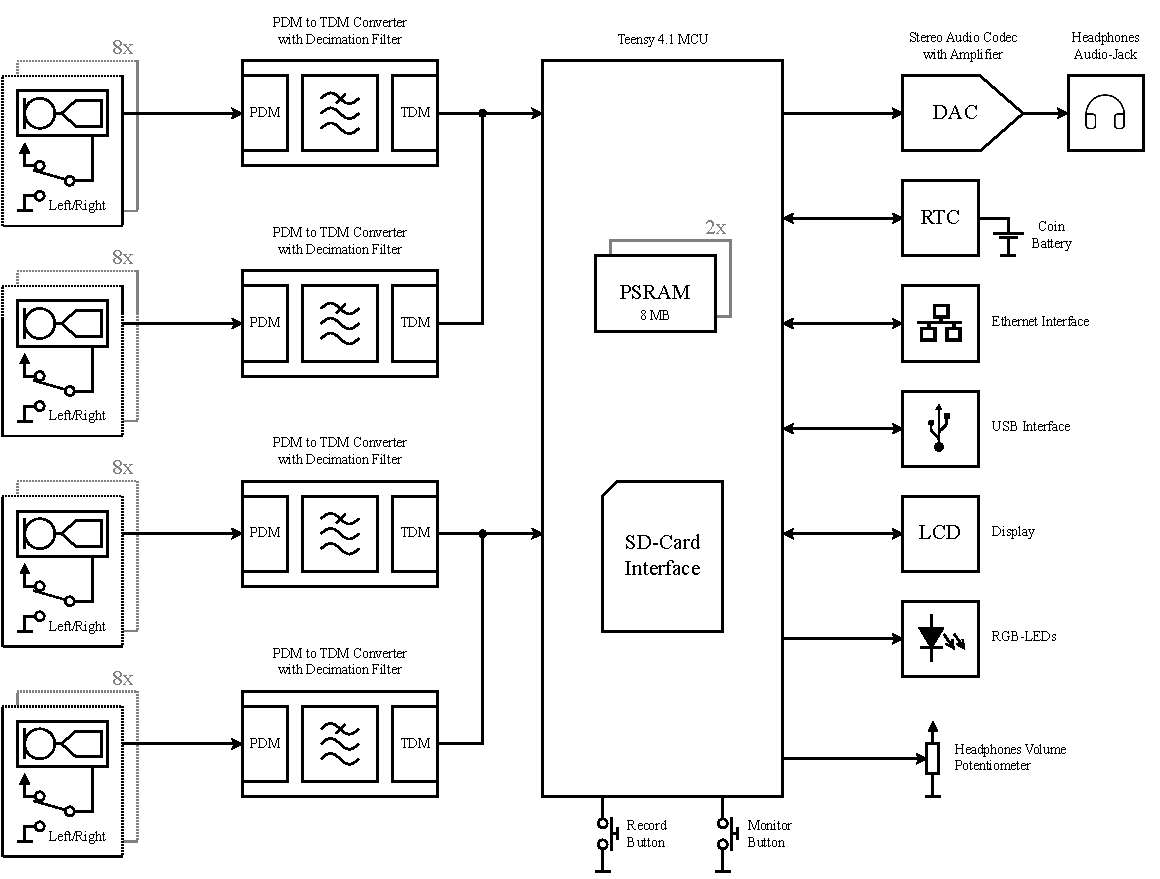
\includegraphics[width=1.0\textwidth]{images/4_design_acquisition_system/acquisition_system_design_block_diagram.pdf}
	\caption{System block diagram of acquisition system}
	\label{fig:acquisition_system_design_block_diagram}
\end{figure}

\subsection{Microphone Evaluation}

\subsection{Mainboard}
\begin{figure}[h]
	\centering
	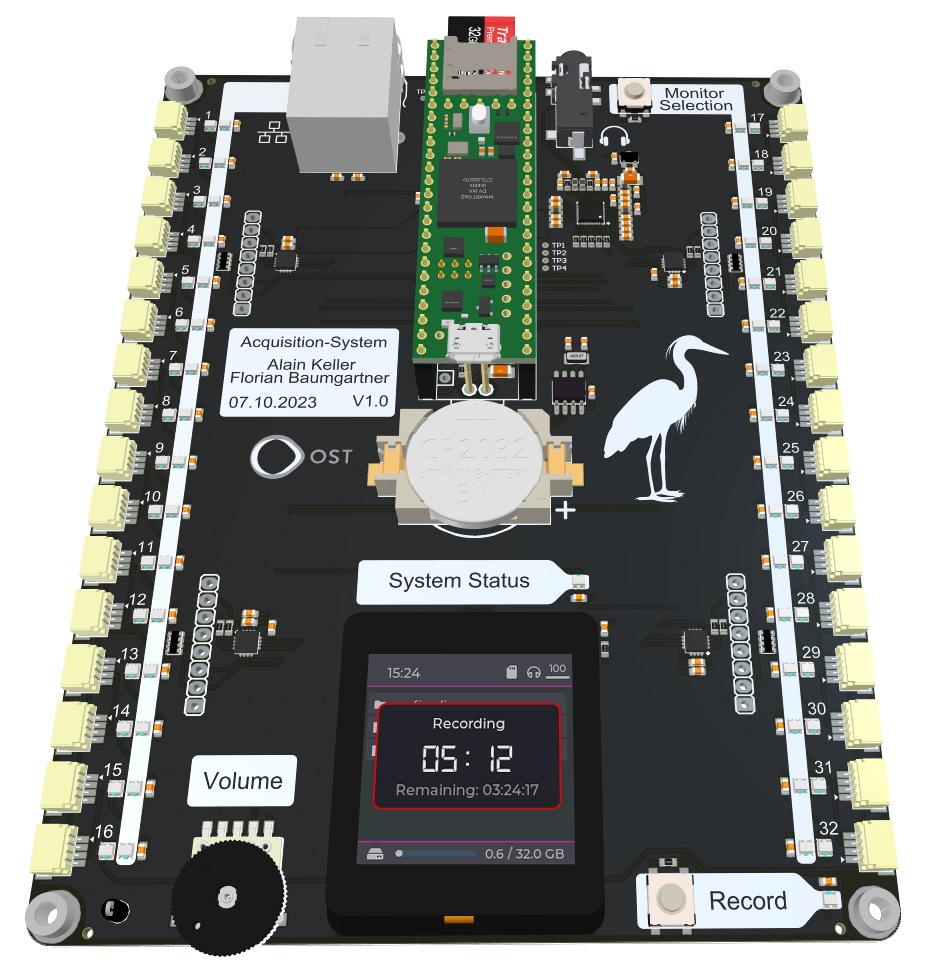
\includegraphics[width=1.0\textwidth]{images/4_design_acquisition_system/Acquisition_System_Front.png}
	\caption{Front view of the Acquisition System}
	\label{fig:acquisition_system_front}
\end{figure}



\subsection{Microcontroller Unit (MCU)}

%  TODO: Write about external PSRAM


\subsection{Audio Input}

\subsection{Headphone Output}

To prelisten the individual audio channels, a headphone output is implemented.

% description of headphones jack
The headphone output is a standard 3.5mm stereo jack.



\newpage
\section{Firmware Design}
Blabla

\subsection{Graphical User Interface (GUI)}

\subsubsection{Light and Versatile Embedded Graphics Library (LVGL)}
LVGL (Light and Versatile Graphics Library) is a free and open-source graphics library, primarily used for creating embedded GUIs (Graphical User Interfaces).
It's designed to be lightweight, consuming minimal memory and processing power, which is essential in embedded systems where resources are limited.

The decision to use LVGL in conjunction with the NXP GuiGuider, a graphical design tool, enables a rich set of features and enables rapid development.
GuiGuider provides a user-friendly interface for designing GUIs, significantly simplifying the process of creating complex, visually appealing interfaces for embedded systems.
It also provides a code generator, which generates the necessary code to initialize and use the GUI in the firmware.

\subsection{GUI Pages}
The \acrshort{gui} is minimalisticly designed and straight forward to use.
The navigation between the main pages is done by swiping left or right on the touchscreen.
Next, the individual pages are described in detail.

\begin{minipage}{\linewidth}
	\begin{wrapfigure}{l}{4.5cm}
		\vspace{-0.6cm}
		
\includegraphics[width=4cm]{images/4_design_acquisition_system/gui/01_splash_screen.png}
		\centering
		\caption{Splash screen}
		\label{fig:acquisition_system_gui_splash_screen}
	\end{wrapfigure}
	\subsubsection{Splash Screen}
	When the device is powered on, the splash screen is displayed until the boot process is finished.
	On average this takes about 5 seconds.
\end{minipage}
\vspace{2.2cm}

\begin{minipage}{\linewidth}
	\begin{wrapfigure}{l}{4.5cm}
		\vspace{-0.6cm}
		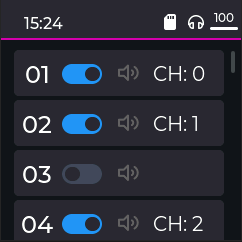
\includegraphics[width=4cm]{images/4_design_acquisition_system/gui/03_channel_settings.png}
		\centering
		\caption{Channel Settings}
		\label{fig:acquisition_system_gui_channel_settings}
	\end{wrapfigure}
	\subsubsection{Channel Settings}
	After the boot process is finished, the channel settings page is displayed.
	In the header bar located at the top of the page, the current time, \acrshort{usb} interface status, SD-Card status and headphones volume are displayed.
	A list of all 32 microphone inputs is shown in the center of the page.
	Each input channel can be enabled or disabled by clicking on the corresponding switch.
	When an input is enabled, its associated channel number of the WAV file is displayed.
	A speaker symbol shows if the channel is currently routed to the headphones monitor output (green means active, grey means inactive).
\end{minipage}
\vspace{0.0cm}

\begin{minipage}{\linewidth}
	\begin{wrapfigure}{l}{4.5cm}
		\vspace{-0.6cm}
		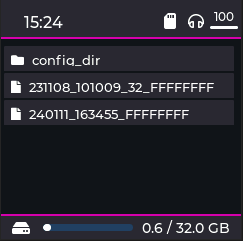
\includegraphics[width=4cm]{images/4_design_acquisition_system/gui/02_file_browser.png}
		\centering
		\caption{File Browser}
		\label{fig:acquisition_system_gui_file_browser}
	\end{wrapfigure}
	\subsubsection{File Browser}
	The file browser shows all files and folders located on the SD-Card.
	On the bottom of the page, a status bar indicates the current free and used space of the SD-Card.
	Due to the limited amount of memory, only the first 100 files and folders are displayed.
	This is however sufficient for most use cases.
\end{minipage}
\vspace{1.8cm}

\begin{minipage}{\linewidth}
	\begin{wrapfigure}{l}{4.5cm}
		\vspace{-0.6cm}
		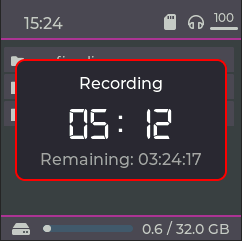
\includegraphics[width=4cm]{images/4_design_acquisition_system/gui/04_recording.png}
		\centering
		\caption{Recording}
		\label{fig:acquisition_system_gui_recording}
	\end{wrapfigure}
	\subsubsection{Recording}
	When the record button is pressed, the recording begins and a panel overlay is displayed.
	In the centre of the panel, the current recording time is displayed in minutes and seconds.
	Below, the remaining recording time is shown.
	When the recording is stopped, the panel overlay disappears.
	While the device is recording, all \acrshort{ui} elements and the navigation are disabled.
\end{minipage}
\vspace{1.8cm}

\begin{minipage}{\linewidth}
	\begin{wrapfigure}{l}{4.5cm}
		\vspace{-0.6cm}
		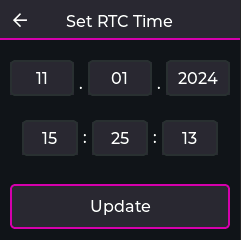
\includegraphics[width=4cm]{images/4_design_acquisition_system/gui/05_set_time.png}
		\centering
		\caption{Set RTC Time}
		\label{fig:acquisition_system_gui_set_time}
	\end{wrapfigure}
	\subsubsection{Set RTC Time}
	When the user clicks on the time in the header bar, the set time page is displayed.
	There the user can set the current time and date.
	After clicking on the \textit{Update} button, the new time is set and the page is closed.
	To abort the process, the user can click on the arrow in the header bar.
\end{minipage}
\vspace{1.8cm}



